% Gabarit pandoc des corrigés publiés (brut et guidé). Contenu sans marque ni nom de site.
% Compilation : lualatex (latexmk -lualatex).
% Le Markdown reste la source unique : ne pas éditer ce fichier .tex à la main.
\documentclass[11pt,a4paper]{article}

% --- Moteur, polices (Latin Modern) et langue ---------------------------------
\usepackage{iftex}
\ifLuaTeX\else\errmessage{Ce document se compile avec lualatex}\fi
\usepackage{amsmath,amssymb,mathtools}
\usepackage{fontspec}
% mathrm=sym : \mathrm prend ses glyphes dans la police mathématique (ℓ, μ, Ω), comme KaTeX.
\usepackage[math-style=TeX,bold-style=TeX,mathrm=sym]{unicode-math}
% Repli pour les glyphes absents de Latin Modern (indices et exposants Unicode,
% flèches, filets des schémas en texte, symboles) : DejaVu, puis Latin Modern Math
% (ℓ, lettres mathématiques Unicode des légendes).
\directlua{
  luaotfload.add_fallback("repliTexte", {"DejaVuSerif:mode=harf;", "DejaVuSans:mode=harf;", "file:latinmodern-math.otf:mode=harf;"})
  luaotfload.add_fallback("repliMono", {"DejaVuSansMono:mode=harf;", "DejaVuSans:mode=harf;", "file:latinmodern-math.otf:mode=harf;"})
}
\setmainfont{Latin Modern Roman}[RawFeature={fallback=repliTexte}]
\setsansfont{Latin Modern Sans}[RawFeature={fallback=repliTexte}]
\setmonofont{Latin Modern Mono}[RawFeature={fallback=repliMono}]
\setmathfont{Latin Modern Math}
\usepackage[french]{babel}
\frenchsetup{SmallCapsFigTabCaptions=false}

% --- Mise en page --------------------------------------------------------------
\usepackage[a4paper,margin=2.2cm,headheight=14pt,footskip=1.2cm]{geometry}
\usepackage{microtype}
\setlength{\emergencystretch}{4em}
\tolerance=1500
\setlength{\parindent}{0pt}
\setlength{\parskip}{0.55\baselineskip plus 2pt minus 1pt}
\usepackage{xcolor}
% Gris nommés : babel-french rend « ! » actif dans le document.
\definecolor{gris2}{gray}{0.98}
\definecolor{gris3}{gray}{0.97}
\definecolor{gris5}{gray}{0.95}
\definecolor{gris35}{gray}{0.65}
\definecolor{gris40}{gray}{0.60}
\definecolor{gris45}{gray}{0.55}
\definecolor{gris50}{gray}{0.50}
\definecolor{gris55}{gray}{0.45}
\definecolor{gris60}{gray}{0.40}
\definecolor{gris65}{gray}{0.35}
\definecolor{gris70}{gray}{0.30}
\definecolor{gris80}{gray}{0.20}
\definecolor{gris85}{gray}{0.15}
\usepackage{graphicx}
\usepackage{float}
\usepackage{caption}
\captionsetup{font=small,labelformat=empty,justification=centering}
\usepackage{booktabs,longtable,array,multirow,calc}
\usepackage{siunitx}
\sisetup{locale=FR}
\usepackage[version=4]{mhchem}
\usepackage{listings}
\usepackage{fancyhdr}
\usepackage{lastpage}
\usepackage[most]{tcolorbox}
\usepackage{enumitem}
\setlist{nosep,leftmargin=*,topsep=2pt}
\usepackage[hidelinks,unicode]{hyperref}
\usepackage{bookmark}
\hypersetup{pdftitle={CCINP TSI — Informatique 2026},pdfauthor={Rédigé par IA},pdfcreator={LaTeX},pdfsubject={Corrigé brut}}
\usepackage{xurl}

% --- Pandoc : listes, tableaux, figures ----------------------------------------
\providecommand{\passthrough}[1]{#1}
\providecommand{\tightlist}{\setlength{\itemsep}{0pt}\setlength{\parskip}{0pt}}

\makeatletter
\def\maxwidth{\ifdim\Gin@nat@width>\linewidth\linewidth\else\Gin@nat@width\fi}
\def\maxheight{\ifdim\Gin@nat@height>0.55\textheight 0.55\textheight\else\Gin@nat@height\fi}
\makeatother
\setkeys{Gin}{width=\maxwidth,height=\maxheight,keepaspectratio}
\setcounter{secnumdepth}{-\maxdimen}
\providecommand{\pandocbounded}[1]{#1}
\usepackage{longtable,booktabs,array}

% --- Code (listings) -----------------------------------------------------------
\lstset{
  basicstyle=\ttfamily\small,
  columns=fullflexible,
  keepspaces=true,
  breaklines=true,
  breakatwhitespace=false,
  postbreak=\mbox{\textcolor{gris50}{$\hookrightarrow$}\space},
  frame=single,
  rulecolor=\color{gris35},
  framesep=4pt,
  xleftmargin=5pt,xrightmargin=5pt,
  backgroundcolor=\color{gris3},
  keywordstyle=\bfseries,
  commentstyle=\color{gris65},
  stringstyle=\color{gris80},
  showstringspaces=false,
  tabsize=4,
  extendedchars=true,
  aboveskip=6pt,belowskip=6pt,
}

% --- Macros des corrigés (KaTeX ↔ LaTeX) ---------------------------------------
% Les corrigés sont écrits pour KaTeX : on définit ici ce que KaTeX connaît et
% que LaTeX n'a pas, sans jamais retoucher le Markdown.
\providecommand{\R}{\mathbb{R}}
\providecommand{\N}{\mathbb{N}}
\providecommand{\Z}{\mathbb{Z}}
\providecommand{\Q}{\mathbb{Q}}
\providecommand{\C}{\mathbb{C}}
\providecommand{\dd}{\mathrm{d}}
\providecommand{\llbracket}{\lBrack}
\providecommand{\rrbracket}{\rBrack}
\providecommand{\lBrace}{\lbrace}
\providecommand{\rBrace}{\rbrace}
\providecommand{\Box}{\square}
\providecommand{\Diamond}{\lozenge}
\providecommand{\varnothing}{\emptyset}
\providecommand{\argmax}{\operatorname*{arg\,max}}
\providecommand{\argmin}{\operatorname*{arg\,min}}
\renewcommand{\leq}{\leqslant}
\renewcommand{\geq}{\geqslant}

% Équation hors texte : réduite à la largeur de la ligne si elle déborde.
\newsavebox{\boiteequation}
\newcommand{\equationajustee}[1]{%
  \sbox{\boiteequation}{$\displaystyle #1$}%
  \ifdim\wd\boiteequation>\linewidth
    \[\resizebox{\linewidth}{!}{\usebox{\boiteequation}}\]%
  \else
    \[#1\]%
  \fi}

% --- Encadrés pédagogiques (sobres, lisibles en noir et blanc) -----------------
\tcbset{
  encadre/.style={
    enhanced,breakable,sharp corners,
    colback=white,colframe=gris55,
    boxrule=0.4pt,leftrule=2.2pt,
    left=6pt,right=6pt,top=3pt,bottom=3pt,
    before skip=6pt,after skip=6pt,
    fonttitle=\bfseries\small,coltitle=black,
    attach title to upper,after title={\quad},
    parbox=false,
  }
}
\newtcolorbox{indication}[1]{encadre,colframe=gris45,colback=gris2,title={Indication~#1}}
\newtcolorbox{methode}{encadre,colframe=gris70,title={Méthode}}
\newtcolorbox{piege}{encadre,colframe=gris85,boxrule=0.8pt,leftrule=2.2pt,title={Piège}}
\newtcolorbox{jury}{encadre,colframe=gris60,colback=gris5,title={Jury}}
\newtcolorbox{encadrenote}{encadre,colframe=gris40}

% --- Titres de section ---------------------------------------------------------
\usepackage{titlesec}
\titleformat{\section}{\Large\bfseries}{}{0pt}{}
\titleformat{\subsection}{\large\bfseries}{}{0pt}{}
\titleformat{\subsubsection}{\normalsize\bfseries}{}{0pt}{}
\titlespacing*{\section}{0pt}{14pt plus 4pt minus 2pt}{6pt}
\titlespacing*{\subsection}{0pt}{10pt plus 3pt minus 2pt}{4pt}
\titlespacing*{\subsubsection}{0pt}{8pt plus 2pt minus 2pt}{2pt}

% --- En-tête et pied de page ---------------------------------------------------
\pagestyle{fancy}
\fancyhf{}
\fancyhead[L]{\small\textsc{Corrigé brut} · CCINP TSI}
\fancyhead[R]{\small Informatique 2026}
\fancyfoot[L]{\footnotesize Corrigé rédigé par IA, non officiel}
\fancyfoot[R]{\footnotesize \thepage\,/\,\pageref*{LastPage}}
\renewcommand{\headrulewidth}{0.4pt}
\renewcommand{\footrulewidth}{0pt}
\fancypagestyle{plain}{\fancyhf{}\fancyfoot[R]{\footnotesize \thepage\,/\,\pageref*{LastPage}}\fancyfoot[L]{\footnotesize Corrigé rédigé par IA, non officiel}\renewcommand{\headrulewidth}{0pt}}

\begin{document}
\thispagestyle{plain}
\begin{center}
  {\small\scshape Corrigé brut}\par\smallskip
  {\LARGE\bfseries CCINP TSI — Informatique 2026\par}\medskip
  {\large CCINP · TSI · Informatique · 2026\par}
\end{center}
\vspace{2pt}\hrule\vspace{8pt}

\emph{Corrigé rédigé par IA, non officiel. Signalez toute erreur.}

Épreuve de 3 heures, calculatrice interdite. Le Document Réponse (DR), qui porte les codes à trous des Q5, Q12, Q16, Q22 et Q23, n'est pas reproduit ici : ces fonctions sont donc écrites en entier, avec les noms, paramètres et valeurs de retour imposés par l'énoncé. Convention : la case \((i, j)\) est celle de la ligne \(i\) et de la colonne \(j\).

\hypertarget{partie-i-des-algorithmes-pour-ruxe9soudre-le-probluxe8me-des-n-reines}{%
\section{Partie I --- Des algorithmes pour résoudre le problème des n reines}\label{partie-i-des-algorithmes-pour-ruxe9soudre-le-probluxe8me-des-n-reines}}

\hypertarget{i.1-introduction}{%
\subsection{I.1 --- Introduction}\label{i.1-introduction}}

\textbf{Q1.} Dans la configuration perdante, les reines occupent les cases (ligne, colonne) \((0,0)\), \((1,2)\), \((2,3)\) et \((3,1)\). Lignes et colonnes sont distinctes.

Deux cases sont sur une même diagonale montante si elles ont la même somme \(i+j\), sur une même diagonale descendante si elles ont la même différence \(i-j\). Ici :

\begin{longtable}[]{@{}lllll@{}}
\toprule\noalign{}
Reine & (0, 0) & (1, 2) & (2, 3) & (3, 1) \\
\midrule\noalign{}
\endhead
\bottomrule\noalign{}
\endlastfoot
\(i+j\) & 0 & 3 & 5 & 4 \\
\(i-j\) & 0 & −1 & −1 & 2 \\
\end{longtable}

Les sommes sont distinctes, mais la différence −1 apparaît deux fois.

\textbf{Les reines des cases \((1,2)\) et \((2,3)\) sont sur la même diagonale descendante (elles sont même diagonalement voisines) : elles se contrôlent mutuellement, la configuration ne résout pas le problème.}

\begin{figure}[H]
\centering
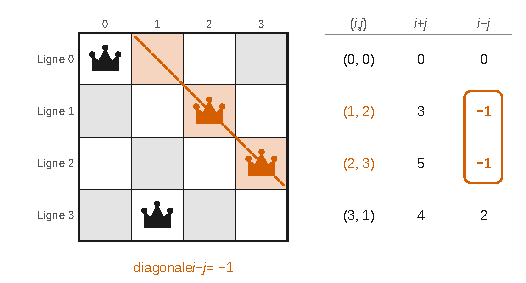
\includegraphics{figures/q1-configuration-perdante.pdf}
\caption*{Figure 1 --- Q1 : dans la configuration perdante, les reines (1, 2) et
(2, 3) partagent la diagonale descendante i − j = −1}
\end{figure}

\textbf{Q2.} On lit, ligne par ligne, la colonne de la reine (contrôle sur la figure 5 : on retrouve bien \texttt{{[}2,\ 4,\ 1,\ 3,\ 0{]}}).

\equationajustee{\boxed{L_{\text{gagnante}} = [2, 0, 3, 1]}}

\equationajustee{\boxed{L_{\text{perdante}} = [0, 2, 3, 1]}}

\hypertarget{i.2-mise-en-place-dun-affichage}{%
\subsection{I.2 --- Mise en place d'un affichage}\label{i.2-mise-en-place-dun-affichage}}

\textbf{Q3.}

\begin{lstlisting}[language=Python]
def ligne(n):
    L = []
    for k in range(n):
        L.append(0)
    return L
\end{lstlisting}

(L'écriture \texttt{return\ {[}0{]}\ *\ n} est également correcte : 0 est un entier, objet non modifiable.)

\textbf{Q4.} Il faut \(n\) listes \textbf{distinctes} en mémoire : on appelle \texttt{ligne(n)} à chaque tour, plutôt que d'écrire \texttt{{[}ligne(n){]}\ *\ n} qui crée \(n\) références vers la même liste.

\begin{lstlisting}[language=Python]
def grille(n):
    G = []
    for i in range(n):
        G.append(ligne(n))
    return G
\end{lstlisting}

\textbf{Q5.} Pour chaque ligne \(i\), une seule case vaut 1 : celle de colonne \texttt{L{[}i{]}}. On l'écrit directement, sans double boucle.

\begin{lstlisting}[language=Python]
def remplir(L):
    n = len(L)
    G = grille(n)
    for i in range(n):
        G[i][L[i]] = 1
    return G
\end{lstlisting}

La boucle de placement effectue \texttt{len(L)} affectations à coût constant : elle est en \(O(\texttt{len(L)})\). (La création de la grille par \texttt{grille(n)} coûte, elle, \(\Theta(n^2)\), ce qui est incompressible pour une grille \(n \times n\).) Sur \texttt{{[}1,\ 3,\ 0,\ 2{]}}, on obtient \texttt{{[}{[}0,\allowbreak{}\ 1,\allowbreak{}\ 0,\allowbreak{}\ 0{]}\allowbreak{},\allowbreak{}\ {[}0,\allowbreak{}\ 0,\allowbreak{}\ 0,\allowbreak{}\ 1{]}\allowbreak{},\allowbreak{}\ {[}1,\allowbreak{}\ 0,\allowbreak{}\ 0,\allowbreak{}\ 0{]}\allowbreak{},\allowbreak{}\ {[}0,\allowbreak{}\ 0,\allowbreak{}\ 1,\allowbreak{}\ 0{]}\allowbreak{}{]}\allowbreak{}}.

\textbf{Q6.}

\begin{lstlisting}[language=Python]
def affiche(G):
    for rangee in G:
        print(rangee)
\end{lstlisting}

La fonction n'a pas de \texttt{return} : elle renvoie \texttt{None} et affiche une ligne de la grille par ligne d'écran.

\hypertarget{i.3-tester-si-une-configuration-est-valide}{%
\subsection{I.3 --- Tester si une configuration est valide}\label{i.3-tester-si-une-configuration-est-valide}}

\textbf{Q7.} Le codage place exactement une reine par ligne (la reine de la ligne \(i\) est en \((i, L[i])\)).

\begin{itemize}
\tightlist
\item
  \textbf{(a)} Deux reines des lignes \(i \neq k\) sont dans la même colonne si et seulement si \(L[i] = L[k]\) : (a) traduit \textbf{au plus une reine par colonne}.
\item
  \textbf{(b)} Le long d'une diagonale montante, on passe de \((i, j)\) à \((i-1, j+1)\) : la somme \(i + j\) est constante, et deux cases sont sur la même diagonale montante si et seulement si elles ont même somme. Avec \(j = L[i]\), (b) traduit \textbf{au plus une reine par diagonale montante}.
\item
  \textbf{(c)} Le long d'une diagonale descendante, on passe de \((i, j)\) à \((i+1, j+1)\) : la différence \(j - i\) est constante. (c) traduit \textbf{au plus une reine par diagonale descendante}.
\end{itemize}

Avec (d), qui assure qu'il y a \(n\) reines, ces conditions disent qu'aucune reine n'en contrôle une autre.

\begin{figure}[H]
\centering
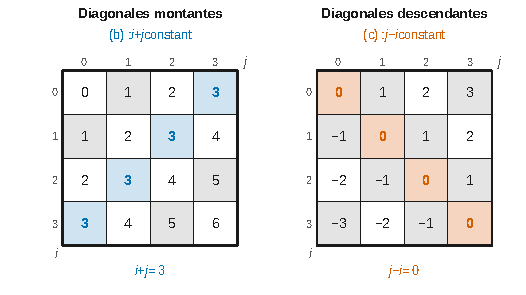
\includegraphics{figures/q7-diagonales-invariants.pdf}
\caption*{Figure 2 --- Q7 : i + j est constant le long d'une diagonale montante, j
− i le long d'une diagonale descendante}
\end{figure}

\textbf{Q8.}

\begin{lstlisting}[language=Python]
def tous_distincts(L):
    presents = dict()
    for x in L:
        if x in presents:
            return False
        presents[x] = True
    return True
\end{lstlisting}

\textbf{Q9.} Deux erreurs : la boucle interne part de \texttt{i} (le couple \((i, i)\) donne toujours une égalité, la fonction renvoie \texttt{True} dès le premier tour pour toute liste non vide) ; les valeurs de retour sont inversées (une égalité prouve qu'il y a un doublon).

\begin{lstlisting}[language=Python]
def tous_distincts2(L):
    n = len(L)
    for i in range(n):
        for j in range(i + 1, n):
            if L[i] == L[j]:
                return False
    return True
\end{lstlisting}

Pire des cas : une liste sans doublon (aucune sortie anticipée).

\begin{itemize}
\tightlist
\item
  \texttt{tous\_distincts} : \(n\) tours, chacun formé d'un test \texttt{x\ in\ presents} et d'une insertion, en \(O(1)\) d'après l'annexe 2 : \textbf{\(O(n)\)}.
\item
  \texttt{tous\_distincts2} : chaque comparaison coûte \(O(1)\), et leur nombre est
  \equationajustee{\sum_{i=0}^{n-1} (n - 1 - i) = \frac{n(n-1)}{2},}
  d'où un coût \textbf{\(O(n^2)\)}.
\end{itemize}

\textbf{La version par dictionnaire est linéaire, la version corrigée par double boucle quadratique} (au prix de \(O(n)\) cases mémoire supplémentaires pour le dictionnaire).

\textbf{Q10.}

\begin{lstlisting}[language=Python]
def est_possible(L):
    montantes = []
    descendantes = []
    for i in range(len(L)):
        montantes.append(L[i] + i)
        descendantes.append(L[i] - i)
    return tous_distincts(L) and tous_distincts(montantes) and tous_distincts(descendantes)
\end{lstlisting}

Coût \(O(\texttt{len(L)})\). La fonction n'impose pas \texttt{len(L)\ ==\ n}, ce qui permet de l'appliquer à des configurations partielles (I.7). Contrôle : pour \texttt{{[}3,\allowbreak{}\ 4,\allowbreak{}\ 1,\allowbreak{}\ 7,\allowbreak{}\ 0,\allowbreak{}\ 6,\allowbreak{}\ 2,\allowbreak{}\ 5{]}\allowbreak{}}, les \texttt{L{[}i{]}\ +\ i} valent \(3, 5, 3, \dots\) : (b) échoue, la fonction renvoie \texttt{False} ; pour \texttt{{[}2,\allowbreak{}\ 4,\allowbreak{}\ 1,\allowbreak{}\ 7,\allowbreak{}\ 0,\allowbreak{}\ 6,\allowbreak{}\ 3,\allowbreak{}\ 5{]}\allowbreak{}}, les trois listes sont sans doublon, elle renvoie \texttt{True}.

\textbf{Q11.}

\begin{lstlisting}[language=Python]
def est_solution(L, n):
    return len(L) == n and est_possible(L)
\end{lstlisting}

\hypertarget{i.4-une-premiuxe8re-approche-par-recherche-aluxe9atoire}{%
\subsection{I.4 --- Une première approche par recherche aléatoire}\label{i.4-une-premiuxe8re-approche-par-recherche-aluxe9atoire}}

\textbf{Q12.} Méthode 1, import du module :

\begin{lstlisting}[language=Python]
import random
P = random.sample(L, len(L))
\end{lstlisting}

Méthode 2, import de la seule fonction, appel direct (celle utilisée ensuite, puisque l'énoncé écrit \texttt{sample(\allowbreak{}L,\allowbreak{}\ len(\allowbreak{}L)\allowbreak{})\allowbreak{}} sans préfixe) :

\begin{lstlisting}[language=Python]
from random import sample
P = sample(L, len(L))
\end{lstlisting}

(Troisième forme au programme : \texttt{import\ random\ as\ rd}, puis \texttt{rd.sample(\allowbreak{}L,\allowbreak{}\ len(\allowbreak{}L)\allowbreak{})\allowbreak{}}.)

\textbf{Q13.}

\begin{lstlisting}[language=Python]
def recherche_aleatoire(n, N):
    L = []
    for i in range(n):
        L.append(i)
    for essai in range(N):
        P = sample(L, len(L))
        if est_solution(P, n):
            return P
    return []
\end{lstlisting}

Le tirage est fait \textbf{dans} la boucle (sinon on testerait \(N\) fois la même liste) ; la valeur d'échec est \texttt{{[}{]}} comme imposé. Coût au pire \(O(nN)\).

\hypertarget{i.5-duxe9terminer-toutes-les-permutations-de-l-0-1-n-1}{%
\subsection{I.5 --- Déterminer toutes les permutations de L = {[}0, 1, \ldots, n-1{]}}\label{i.5-duxe9terminer-toutes-les-permutations-de-l-0-1-n-1}}

\textbf{Q14.}

\begin{lstlisting}[language=Python]
def insertion(x, L, i):
    M = []
    for k in range(i):
        M.append(L[k])
    M.append(x)
    for k in range(i, len(L)):
        M.append(L[k])
    return M
\end{lstlisting}

\texttt{insertion(\allowbreak{}5,\allowbreak{}\ {[}2,\allowbreak{}\ 3,\allowbreak{}\ 6,\allowbreak{}\ 4{]}\allowbreak{},\allowbreak{}\ 1)\allowbreak{}} renvoie \texttt{{[}2,\ 5,\ 3,\ 6,\ 4{]}} et \texttt{insertion(\allowbreak{}5,\allowbreak{}\ {[}2,\allowbreak{}\ 3,\allowbreak{}\ 6,\allowbreak{}\ 4{]}\allowbreak{},\allowbreak{}\ 4)\allowbreak{}} renvoie \texttt{{[}2,\ 3,\ 6,\ 4,\ 5{]}} ; la liste \texttt{L} n'est pas modifiée.

Seule une fonction d'insertion toute faite (comme \texttt{L.insert}) est interdite : le découpage en tranches est permis, et \texttt{return\ L{[}:\allowbreak{}i{]}\allowbreak{}\ +\ {[}x{]}\allowbreak{}\ +\ L{[}i:\allowbreak{}{]}\allowbreak{}} est une réponse équivalente.

\textbf{Q15.} À l'issue du premier passage dans la boucle externe (\texttt{l1\ =\ {[}0,\ 1{]}}, \(i = 0, 1, 2\)) :

\equationajustee{\boxed{P = [[2, 0, 1],\ [0, 2, 1],\ [0, 1, 2]]}}

(Si l'on comprend « premier passage » comme le premier tour de la boucle interne, \texttt{P} vaut alors \texttt{{[}{[}2,\ 0,\ 1{]}{]}}.) Après exécution complète, le second passage (\texttt{l1\ =\ {[}1,\ 0{]}}) ajoute trois listes :

\equationajustee{\boxed{P = [[2, 0, 1],\ [0, 2, 1],\ [0, 1, 2],\ [2, 1, 0],\ [1, 2, 0],\ [1, 0, 2]]}}

\textbf{Ce code construit toutes les permutations de \(\{0, 1, 2\}\) à partir de celles de \(\{0, 1\}\) : il insère la nouvelle valeur \(v = 2\) à chacune des \(v + 1 = 3\) positions possibles de chaque permutation de \texttt{L}.}

Il n'y a ni oubli ni doublon : en retirant le 2 d'une permutation de \(\{0, 1, 2\}\), on retrouve une unique permutation de \(\{0, 1\}\) et une unique position d'insertion. On obtient bien \(2 \times 3 = 3!\) listes.

\begin{figure}[H]
\centering
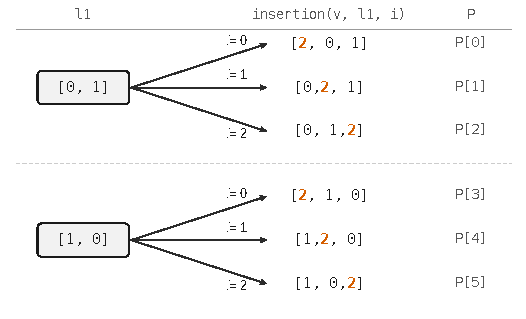
\includegraphics{figures/q15-insertion-permutations.pdf}
\caption*{Figure 3 --- Q15 : chaque permutation l1 de \{0, 1\} donne trois listes
insertion(v, l1, i) avec v = 2, rangées dans P dans l'ordre}
\end{figure}

\textbf{Q16.} On répète le procédé de la Q15 pour \(v = 2, 3, \dots, n-1\), en repartant chaque fois de la liste obtenue à l'étape précédente.

\begin{lstlisting}[language=Python]
def permutations(n):
    P = [[0, 1], [1, 0]]
    for v in range(2, n):
        Q = []
        for l1 in P:
            for i in range(v + 1):
                Q.append(insertion(v, l1, i))
        P = Q
    return P
\end{lstlisting}

Par récurrence sur \(v\) : avant le tour d'indice \(v\), \texttt{P} contient sans répétition les \(v!\) permutations de \(\{0, \dots, v-1\}\). L'argument de la Q15 montre qu'après le tour, \texttt{P} contient les \((v+1)!\) permutations de \(\{0, \dots, v\}\).

En sortie, \texttt{P} contient donc les \(n!\) permutations de \(\{0, \dots, n-1\}\). Pour \(n = 2\), la boucle est vide et la fonction renvoie \texttt{{[}{[}0,\ 1{]},\ {[}1,\ 0{]}{]}}.

\texttt{permutations(3)} renvoie \texttt{{[}{[}2,\allowbreak{}\ 0,\allowbreak{}\ 1{]}\allowbreak{},\allowbreak{}\ {[}0,\allowbreak{}\ 2,\allowbreak{}\ 1{]}\allowbreak{},\allowbreak{}\ {[}0,\allowbreak{}\ 1,\allowbreak{}\ 2{]}\allowbreak{},\allowbreak{}\ {[}2,\allowbreak{}\ 1,\allowbreak{}\ 0{]}\allowbreak{},\allowbreak{}\ {[}1,\allowbreak{}\ 2,\allowbreak{}\ 0{]}\allowbreak{},\allowbreak{}\ {[}1,\allowbreak{}\ 0,\allowbreak{}\ 2{]}\allowbreak{}{]}\allowbreak{}}. Coût \(\Theta(n \cdot n!)\).

\textbf{Q17.}

\begin{lstlisting}[language=Python]
def configurations(n):
    C = []
    for p in permutations(n):
        if est_solution(p, n):
            C.append(p)
    return C
\end{lstlisting}

Toute solution est une liste de \(n\) entiers distincts de \(\{0, \dots, n-1\}\), donc une permutation : elle est produite par \texttt{permutations(n)} et retenue ; réciproquement, toute liste retenue vérifie (a), (b), (c), (d). On retrouve 10 configurations pour \(n = 5\) et 92 pour \(n = 8\).

\hypertarget{i.6-classer-les-configurations-similaires}{%
\subsection{I.6 --- Classer les configurations similaires}\label{i.6-classer-les-configurations-similaires}}

\textbf{Q18.} Avec \(L = [2, 4, 1, 3, 0]\) et \(n = 5\).

\begin{itemize}
\tightlist
\item
  Symétrie horizontale (axe horizontal) : les lignes \(i\) et \(n - 1 - i\) sont échangées, les colonnes inchangées. La reine de la ligne \(i\) passe en ligne \(n-1-i\), même colonne, donc \(L_1[i] = L[n-1-i]\).
\end{itemize}

\equationajustee{\boxed{L_1 = [0, 3, 1, 4, 2]}}

\begin{itemize}
\tightlist
\item
  Rotation d'un quart de tour vers la droite : la reine \((i, L[i])\) passe en \((L[i], n-1-i)\), donc \(L_2[L[i]] = n - 1 - i\). Pour \(i = 0, \dots, 4\) :
\end{itemize}

\equationajustee{\begin{aligned}
L_2[2] &= 4 \\
L_2[4] &= 3 \\
L_2[1] &= 2 \\
L_2[3] &= 1 \\
L_2[0] &= 0
\end{aligned}}

\equationajustee{\boxed{L_2 = [0, 2, 4, 1, 3]}}

Ces deux listes correspondent aux grilles de la figure 6. \textbf{De façon générale, \(L_1\) est la liste \(L\) lue à l'envers : \(L_1[i] = L[n-1-i]\) pour \(0 \le i \le n-1\).}

\begin{figure}[H]
\centering
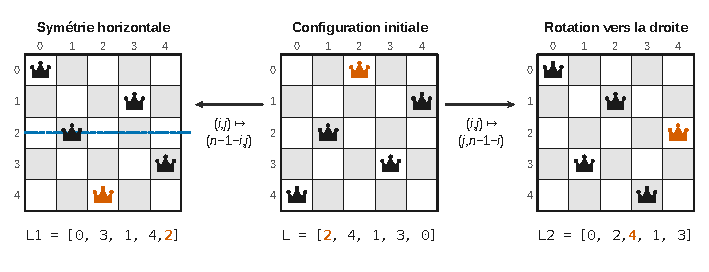
\includegraphics{figures/q18-symetrie-rotation.pdf}
\caption*{Figure 4 --- Q18 : symétrie horizontale et rotation vers la droite de la
configuration initiale, en suivant la reine de la ligne 0}
\end{figure}

\textbf{Q19.}

\begin{lstlisting}[language=Python]
def symetrie(L):
    n = len(L)
    M = []
    for i in range(n):
        M.append(L[n - 1 - i])
    return M
\end{lstlisting}

\texttt{symetrie(\allowbreak{}{[}1,\allowbreak{}\ 0,\allowbreak{}\ 2{]}\allowbreak{})\allowbreak{}} renvoie \texttt{{[}2,\ 0,\ 1{]}}.

\textbf{Q20.} La nouvelle liste se remplit à l'indice \texttt{L{[}i{]}}, et non dans l'ordre : on crée d'abord \(n\) cases.

\begin{lstlisting}[language=Python]
def rotation(L):
    n = len(L)
    M = ligne(n)
    for i in range(n):
        M[L[i]] = n - 1 - i
    return M
\end{lstlisting}

Comme \(L\) est une permutation de \(\{0, \dots, n-1\}\), chaque case de \texttt{M} est écrite exactement une fois. \texttt{rotation(\allowbreak{}{[}2,\allowbreak{}\ 5,\allowbreak{}\ 3,\allowbreak{}\ 1,\allowbreak{}\ 7,\allowbreak{}\ 4,\allowbreak{}\ 6,\allowbreak{}\ 0{]}\allowbreak{})\allowbreak{}} renvoie \texttt{{[}0,\allowbreak{}\ 4,\allowbreak{}\ 7,\allowbreak{}\ 5,\allowbreak{}\ 2,\allowbreak{}\ 6,\allowbreak{}\ 1,\allowbreak{}\ 3{]}\allowbreak{}}.

\textbf{Q21.}

\begin{itemize}
\tightlist
\item
  \textbf{Ligne 1} : \texttt{C\ =\allowbreak{}\ configurations(\allowbreak{}n)\allowbreak{}} place dans \texttt{C} la liste de toutes les configurations solutions du problème pour une grille \(n \times n\) (Q17).
\item
  \textbf{Type renvoyé} : \texttt{partition(n)} renvoie \textbf{une liste}.
\item
  \textbf{Structure} : c'est une \textbf{liste de listes de configurations}, c'est-à-dire une liste de listes de listes d'entiers. \texttt{P} est la liste des classes ; chaque classe \texttt{elt} est une liste non vide de configurations deux à deux similaires ; chaque configuration est une liste de \(n\) entiers. Le premier élément \texttt{elt{[}0{]}} d'une classe est la première configuration de \texttt{C} rangée dans cette classe ; il sert de représentant.
\item
  \textbf{Fonctionnement} : \textbf{la fonction range les configurations solutions une à une dans des classes de configurations similaires : chaque configuration est comparée au premier élément de chaque classe déjà formée ; elle rejoint la classe dont elle est similaire, et ouvre une nouvelle classe si elle n'est similaire à aucune.} La fonction renvoie la liste de ces classes, qui forment une partition de l'ensemble des solutions.
\end{itemize}

La similarité est une relation d'équivalence (les rotations et symétries du carré forment un groupe) : comparer au seul représentant suffit, et une configuration ne peut pas être similaire à deux représentants distincts (ils seraient similaires entre eux et le second n'aurait pas ouvert de classe). Pour \(n = 5\) on obtient 2 classes (8 et 2 configurations), pour \(n = 8\) 12 classes (onze de 8 et une de 4).

\hypertarget{i.7-des-graphes-pour-aller-plus-vite-et-plus-loin}{%
\subsection{I.7 --- Des graphes pour aller plus vite et plus loin}\label{i.7-des-graphes-pour-aller-plus-vite-et-plus-loin}}

\textbf{Q22.} Les sommets du graphe sont les configurations partielles (listes de longueur \(k\) au niveau \(k\)) ; on le parcourt en profondeur, récursivement, en élaguant dès qu'une configuration partielle est invalide. La liste courante sert de pile (\texttt{append} pour poser une reine, \texttt{pop} pour revenir en arrière). La signature \texttt{explore(L,\ n)} est une hypothèse, le DR n'étant pas disponible.

\begin{lstlisting}[language=Python]
def explore(L, n):
    if len(L) == n:
        return L
    for j in range(n):
        L.append(j)
        if est_possible(L):
            R = explore(L, n)
            if R != -1:
                return R
        L.pop()
    return -1

def resout_graphe(n):
    return explore([], n)
\end{lstlisting}

Correction (récurrence sur \(n - \texttt{len(L)}\)) : si \texttt{L} est une configuration partielle valide, \texttt{explore(L,\ n)} renvoie une solution prolongeant \texttt{L} s'il en existe, et \(-1\) sinon, en laissant \texttt{L} intacte en cas d'échec. En effet, toute solution prolongeant \texttt{L} commence par \texttt{L\ +\ {[}j{]}} pour un \(j\), et \texttt{L\ +\ {[}j{]}} est alors valide (un préfixe d'une configuration valide est valide) : la boucle examine tous les \(j\), l'élagage ne supprime aucune solution, et chaque \texttt{append} est défait par un \texttt{pop} en cas d'échec. Terminaison : \(n - \texttt{len(L)}\) décroît strictement à chaque appel, la profondeur est au plus \(n\). On obtient \texttt{resout\_graphe(\allowbreak{}4)\allowbreak{}\ =\allowbreak{}\ {[}1,\allowbreak{}\ 3,\allowbreak{}\ 0,\allowbreak{}\ 2{]}\allowbreak{}} et \texttt{resout\_graphe(\allowbreak{}8)\allowbreak{}\ =\allowbreak{}\ {[}0,\allowbreak{}\ 4,\allowbreak{}\ 7,\allowbreak{}\ 5,\allowbreak{}\ 2,\allowbreak{}\ 6,\allowbreak{}\ 1,\allowbreak{}\ 3{]}\allowbreak{}}.

\begin{figure}[H]
\centering
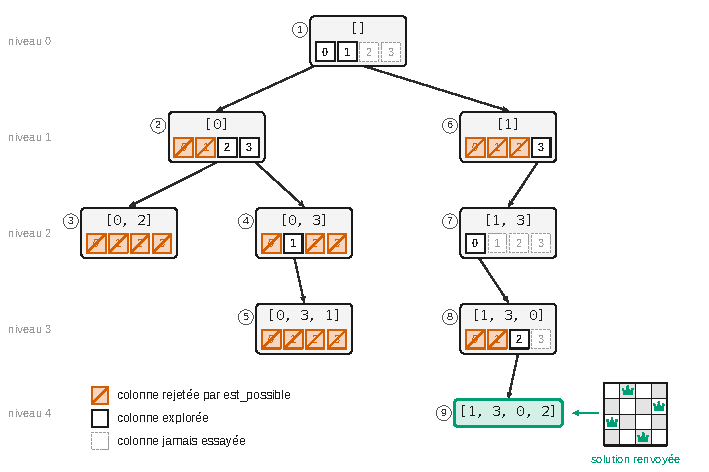
\includegraphics{figures/q22-retour-sur-trace.pdf}
\caption*{Figure 5 --- Q22 : configurations partielles visitées par explore pour n
= 4, colonnes rejetées par l'élagage, arrêt à la première solution}
\end{figure}

\textbf{Q23.} On ne s'arrête plus à la première solution : on renvoie 1 pour une configuration complète et on additionne les résultats des sous-arbres.

\begin{lstlisting}[language=Python]
def explore2(L, n):
    if len(L) == n:
        return 1
    total = 0
    for j in range(n):
        L.append(j)
        if est_possible(L):
            total = total + explore2(L, n)
        L.pop()
    return total

def compte(n):
    return explore2([], n)
\end{lstlisting}

Par la même récurrence, \texttt{explore2(L,\ n)} renvoie le nombre de solutions prolongeant la configuration partielle valide \texttt{L} : ces prolongements se répartissent, sans recouvrement, selon la colonne \(j\) de la reine suivante. On obtient \texttt{compte(4)\ =\ 2}, \texttt{compte(5)\ =\ 10}, \texttt{compte(8)\ =\ 92}, en accord avec la Q17.

\hypertarget{partie-ii-base-de-donnuxe9es-dun-serveur-de-jeu-en-ligne}{%
\section{Partie II --- Base de données d'un serveur de jeu en ligne}\label{partie-ii-base-de-donnuxe9es-dun-serveur-de-jeu-en-ligne}}

\textbf{Q24.} Le format est \texttt{\textquotesingle{}JJ-MM\textquotesingle{}} : le 3 juillet s'écrit \texttt{\textquotesingle{}03-07\textquotesingle{}}.

\begin{lstlisting}[language=SQL]
SELECT nom, prenom, email
FROM Clients
WHERE anniversaire = '03-07';
\end{lstlisting}

Sur l'extrait de l'annexe 1, la requête renvoie Jean Dupont et Tom Cruise.

\textbf{Q25.}

\begin{lstlisting}[language=SQL]
SELECT Clients.nom, Clients.prenom, Factures.date_achat
FROM Clients
JOIN Factures ON Clients.id_client = Factures.id_client
WHERE Clients.email = 'myriam.sarr@ccinp.edu';
\end{lstlisting}

Une ligne par achat du client.

\begin{figure}[H]
\centering
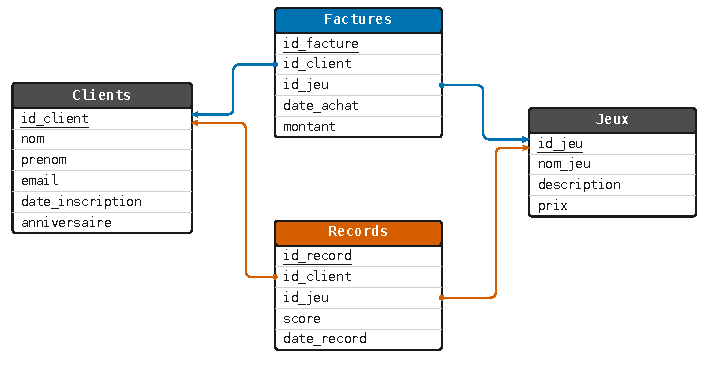
\includegraphics{figures/partie2-schema-relationnel.pdf}
\caption*{Figure 6 --- Partie II : schéma de la base, clés primaires soulignées,
flèches des clés étrangères vers les clés qu'elles référencent}
\end{figure}

\textbf{Q26.} On groupe par la clé primaire du client (deux homonymes ne doivent pas être confondus).

\begin{lstlisting}[language=SQL]
SELECT Clients.nom, Clients.email, SUM(Factures.montant) AS total
FROM Clients
JOIN Factures ON Clients.id_client = Factures.id_client
GROUP BY Clients.id_client, Clients.nom, Clients.email;
\end{lstlisting}

La jointure interne ne fait apparaître que les clients ayant au moins un achat ; un client sans facture, dont le total serait nul, n'est pas listé.

\textbf{Q27.}

\begin{lstlisting}[language=SQL]
SELECT Jeux.nom_jeu, MAX(Records.score) AS meilleur_score
FROM Jeux
JOIN Records ON Jeux.id_jeu = Records.id_jeu
GROUP BY Jeux.id_jeu, Jeux.nom_jeu;
\end{lstlisting}

Une ligne par jeu ayant au moins un record, avec le score maximal enregistré pour ce jeu.

\textbf{FIN}

\end{document}
